\documentclass{article}

\usepackage[margin=1in]{geometry}
\usepackage{graphicx}
\usepackage{hyperref}

\title{Work Trial Results}
\author{Emi Soroka}
\date{\today}

\begin{document}
	\maketitle
	\section{Running the code}
	I use \href{https://docs.marimo.io/getting_started/index.html}{marimo} Python notebooks, which are \verb|.py| files that can be run standalone or as notebooks.
	
	To set up marimo:
	\begin{verbatim}
		pip install marimo
		marimo edit task1.py
	\end{verbatim}
	\vspace{-1em}
	Marimo provides advantages over Jupyter because it uses a computational graph to track dependencies and automatically re-run dependent cells after changes are made, preventing out-of-order execution and unreproducible notebook results. It's also  easier to version control.
	
	\section{Task 1} Construct and code the linear OW model and nonlinear AFS model, and visualize the distribution of price impact based on the given data.
	\vspace{-1em}
	\section*{Results} (Figure \ref{fig:task1}.) I used the provided data with the following preprocessing: data was binned into 10 second intervals using Pandas to aggregate it, and the signed volume was used for $\dot Q$. This followed an example in the Handbook of Price Impact Modeling. I did not remove the after hours trades from the data.
	
	\begin{figure}[h]
		\centering
		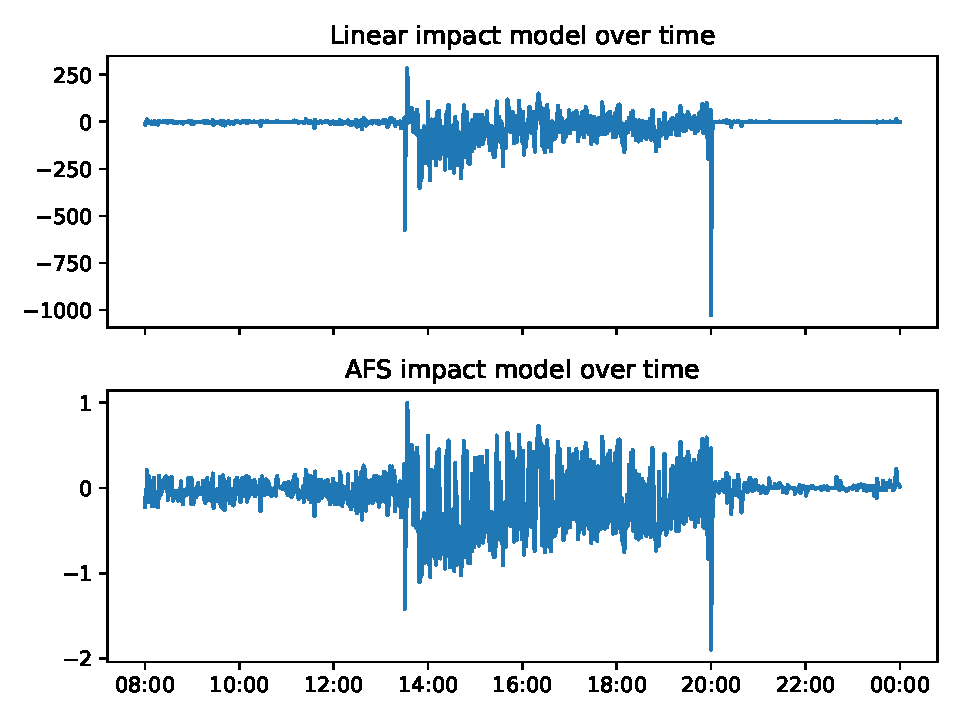
\includegraphics[width=0.6\linewidth]{figures/task1.pdf}
		\caption{Price impact computed from \texttt{merged\_data.csv}.}
		\label{fig:task1}
	\end{figure}
	
	The AFS model yields a smaller price impact for the same $\beta$ and $\lambda$ parameters, and smooths out the impact of large spikes in signed volume. This makes sense since AFS is a concave model, thus it penalizes larger trades less per share than mid-sized trades.
	
	\section{Task 2}
	Implement and code the optimal strategy with Linear Impact and visualize the Sharpe Ratio
	plots in Section 6.2.
	\vspace{-1em}
	\section*{Results}
	The results look similar but are off by a scaling factor (Figure \ref{fig:task2}). This is probably caused by confusion on how the paper defines daily risk, which seems to scale with the number of shares, vs PnL.
	
	\begin{figure}[h]
		\centering
		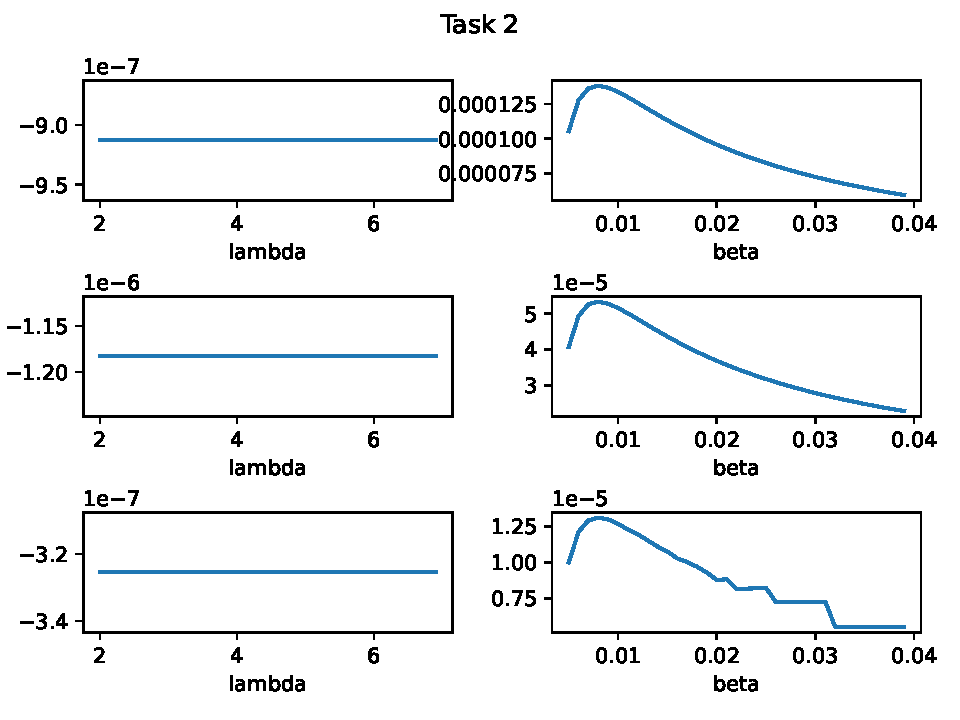
\includegraphics[width=0.6\linewidth]{figures/task2.pdf}
		\caption{Plots generated by optimal strategy. Plots follow the expected shape, however they are off by a scaling factor. The expected behavior of a decrease as the risk increases is still observed.}
		\label{fig:task2}
	\end{figure}
	
	\section{Task 3}
	Implement and code the Deep Learning Algorithm in for discrete setting in Appendix C.2 and visualize the training loss for different network structures in Appendix C.2.
	\vspace{-1em}
	\section*{Results}
	I implemented the deep learning algorithm for the linear model (NetSimple) in Equation C.18 and the linear model (NetLinear). I didn't implement the NetPower modification due to time constraints. In my implementation, NetSimple performed better than NetLinear (Figure \ref{fig:networks}).
	
	\par Because the paper implements a custom environment, defining the signal $f_n$ (Figure \ref{fig:fns}) for the neural network as well as the relationships between $f_n$, $Q_n$ and $J_n^\theta$, I implemented the policy gradient algorithm in my code including rollouts of the policy $\theta$ on batches of signals.
	\vspace{4em}

	\begin{figure}[t]
		\centering
		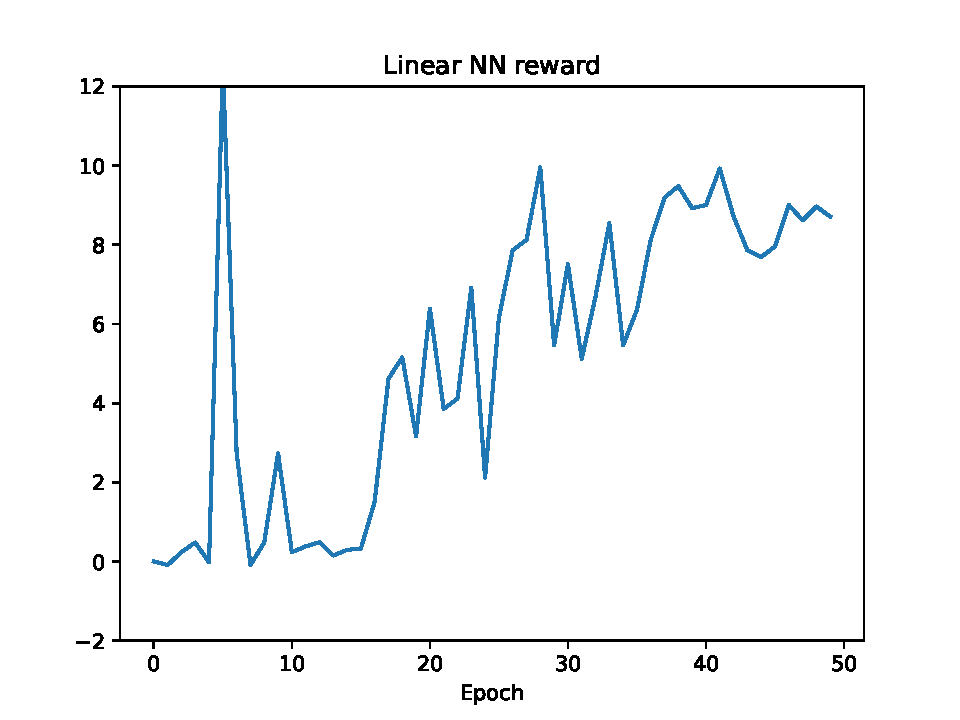
\includegraphics[width=0.49\linewidth]{figures/linear_training_reward.pdf}
		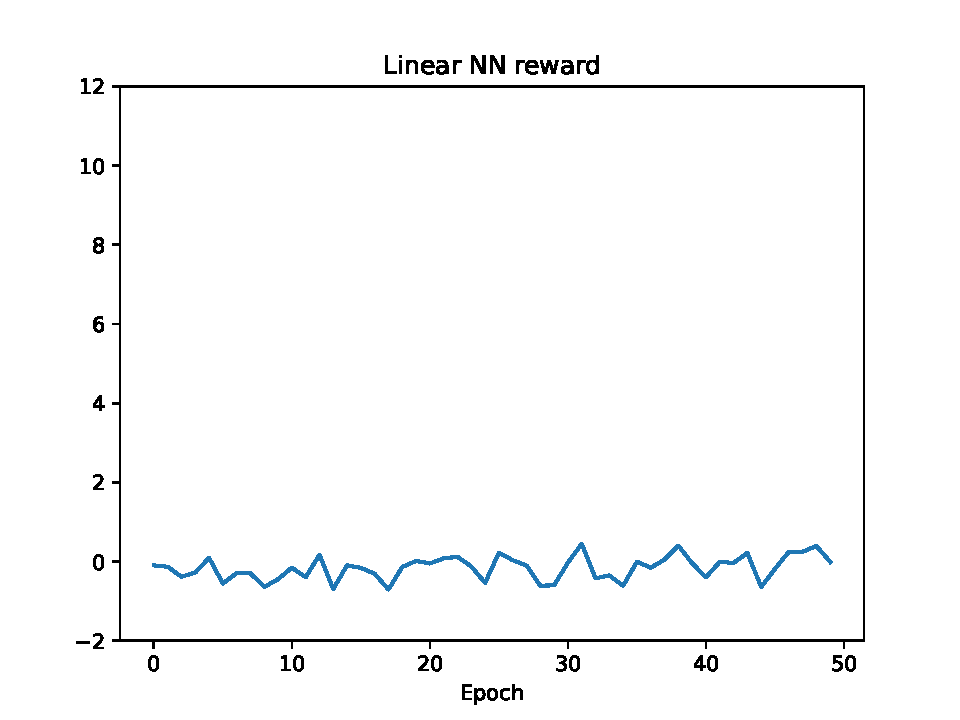
\includegraphics[width=0.49\linewidth]{figures/singlelayer.pdf}
		\caption{Reward function for NetSimple model (left) and single-layer model (right).}
		\label{fig:networks}
	\end{figure}
	
	
	Unfortunately my code is slow; it should be parallelized but I don't have time to do it. I also don't have GPUs available on my computer, and observed that about 50\% of the computational time was due to backpropagation so I concluded the benefit of optimizing the code would be limited.
	Due to this, I used a smaller batch size but the same number of 50 epochs.
	
	\begin{figure}[h]
		\centering
		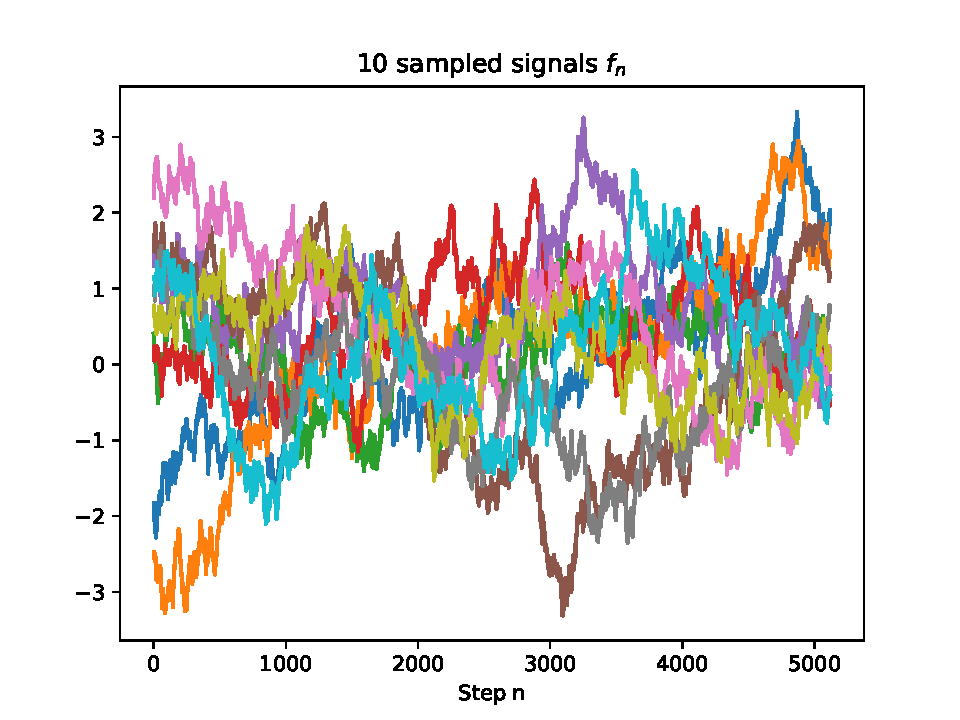
\includegraphics[width=0.5\linewidth]{figures/f1_sample.pdf}
		\caption{Visualization of random samples $\{f_n\}.$}
	\end{figure}
	
\end{document}